The algorithm was executed for 20 iterations using four parallel processes
(\texttt{--ncores 4}). The final prototypes exhibited clear thematic
specialisation.

\begin{table}[h!]
\centering
\begin{tabular}{lll}
\toprule
\textbf{Cluster} & \textbf{Top Attributes (Stemmed)} & \textbf{Inferred Topic} & \textbf{Inferred source}\\
\midrule
CLASS0 & how , inform, import, understand, understand & General Research & --\\
CLASS1 & equat, theori, solut, deriv, space & Mathematics & \texttt{math.update/hep-th}]\\
CLASS2 & quantum, phase, physic, experiment, transit & Quantum Physics & \texttt{quant-ph/cond-mat}\\
CLASS3 & increas, temperatur, investig, valu, found & Thermodynamics & \texttt{cond-mat}\\
CLASS4 & prove, ani, given, bound, some, known & Theoretical CS/Math & \texttt{cs.updates/math}\\
CLASS5 & learn, network, train, deep, dataset & Machine Learning & \texttt{cs.updates}\\
CLASS6 & mass, star, galaxi, stellar, emiss & Astrophysics & \texttt{astro-ph}\\
CLASS7 & optim, effici, bound, linear, complex & Optimisation & \texttt{cs.updates}\\
\bottomrule
\end{tabular}
\caption{Top attributes and thematic labels for selected clusters.}
\end{table}

The computational performance showed significant variance across iterations.
While the first iteration took 2.88 seconds, subsequent iterations' execution times
steadily increased from 2.88 seconds to a maximum of 11.99 seconds.

This increase is attributed to thermal throttling on the
host hardware, which lacked active cooling and reached temperatures in excess
of 100°C during the workload.

\begin{figure}[h!]
\centering
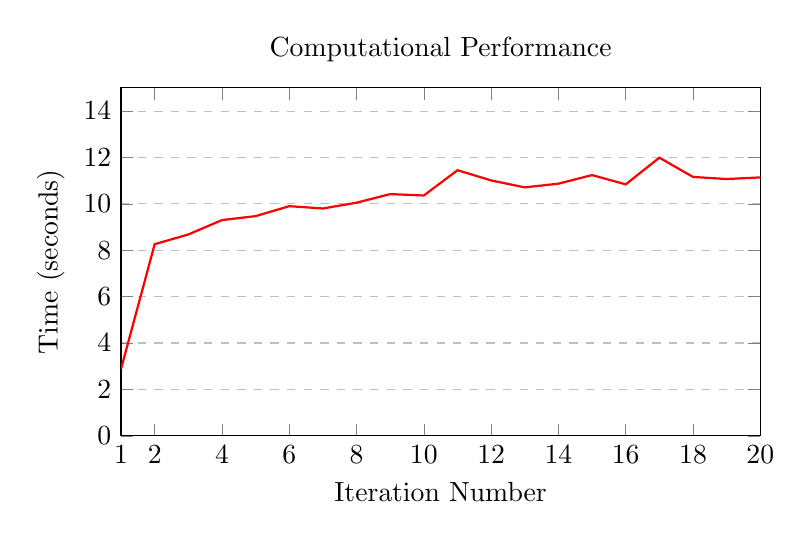
\begin{tikzpicture}
\begin{axis}[
    title={Computational Performance},
    xlabel={Iteration Number},
    ylabel={Time (seconds)},
    xmin=1, xmax=20,
    ymin=0, ymax=15,
    xtick={1,2,4,6,8,10,12,14,16,18,20},
    ytick={0,2,4,6,8,10,12,14},
    legend pos=south east,
    ymajorgrids=true,
    grid style=dashed,
    width=0.8\textwidth,
    height=6cm
]

\addplot[
    color=red,
    mark=circle,
    thick
    ]
    coordinates {
    (1,2.88)(2,8.26)(3,8.68)(4,9.30)(5,9.47)(6,9.90)(7,9.8)(8,10.05)
    (9,10.42)(10,10.36)(11,11.45)(12,11.01)(13,10.71)(14,10.87)(15,11.24)
    (16,10.84)(17,11.99)(18,11.16)(19,11.07)(20,11.14)
    };

\end{axis}
\end{tikzpicture}
\caption{Processing time for each of the 20 K-means iterations. The increase
in execution time observed indicates that from iteration 2 onwards, the CPU
temperature reaches its 100--101°C limit, triggering thermal throttling.}
\label{fig:time_per_iteration}
\end{figure}

As illustrated in Fig.~\ref{fig:time_per_iteration}, the execution time per iteration did not follow the
expected pattern of initial overhead followed by stability.
Instead, a sharp increase in running time was observed starting at Iteration 2,
coinciding with the CPU reaching its thermal limit of 100--101°C.
The computation time steadily increases as the primary cooling thermal mass
(laptop's cooling chamber) is saturated, but the secondary thermal mass
(laptop chassis) begins to absorb heat, leading to a further gradual performance
degradation as the CPU increasingly throttles further to manage temperature.